\section{Data}
The data used in this study were generated by P. Furth et al. in 2023
\supercite{furth_esr1_2023,furth_overexpression_2023}.

\subsection{Mouse models}
Mouse models allow the study of disease pathophysiology within the context of
physiological endocrine and immunologic function.

\subsection{Samples}
Describe the samples used in the study and how they were collected.
Include the timeline plots from the poster.
Explain the different sequencing steps.

\section{Nextflow and nf-core}
\paragraph{Nextflow} is a workflow management system that enables the
development of reproducible and scalable workflows. It allows the creation of
complex pipelines that can be executed on a variety of platforms, from local
machines to cloud computing environments. Nextflow uses a domain-specific
language (DSL) that simplifies the definition of workflows and enables the reuse
of existing components \supercite{di_tommaso_nextflow_2017}. As a result,
Nextflow has become a popular tool in the bioinformatics community.

\begin{figure}[ht]
    \centering
    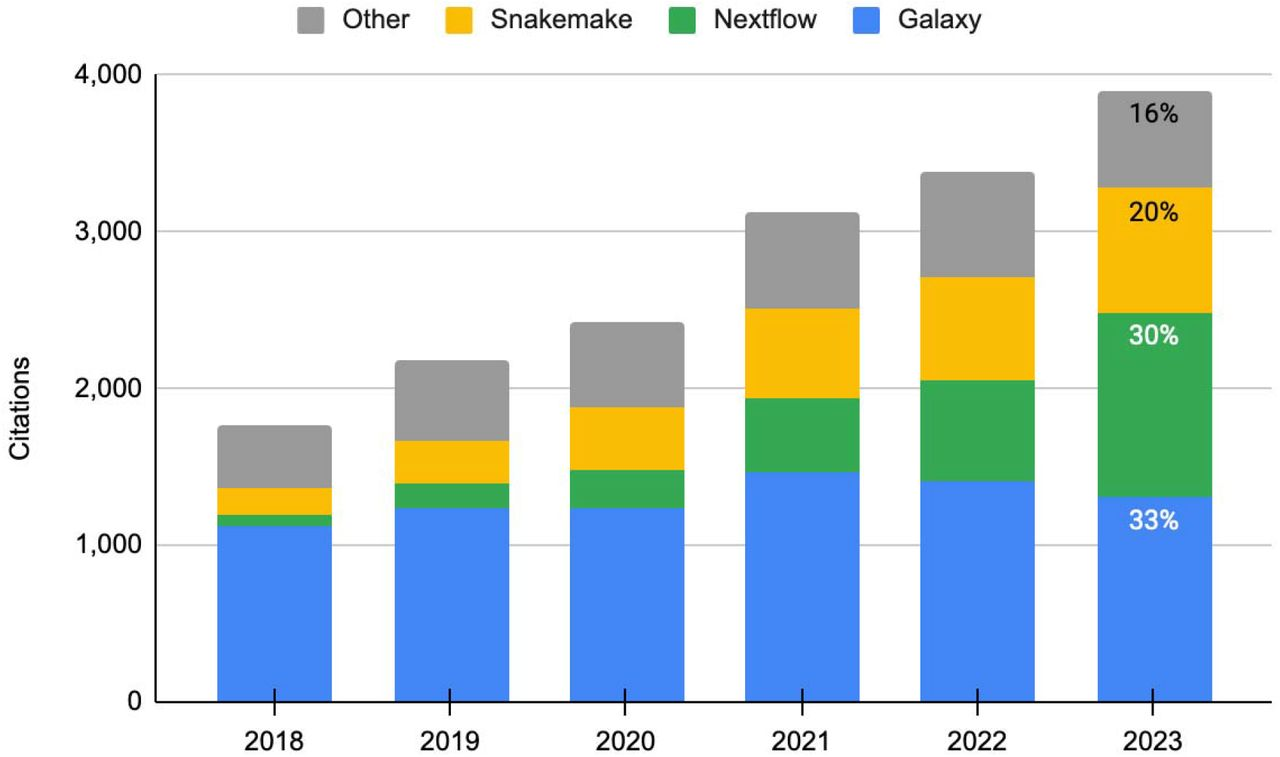
\includegraphics[width=\textwidth]{chapters/materials_and_methods/figures/nextflow_usage.jpg}
    \caption{Workflow management systems} % TODO: Add detailed caption
    \label{fig:nextflow_usage}
\end{figure}

As pointed out by Langer et al. in a recent preprint
\supercite{langer_empowering_2024}, programming-based workflow systems like
Nextflow and Snakemake have gained popularity during the last years, while
GUI-based systems like Galaxy have lost ground. Furthermore, Nextflow has been
the fastest growing workflow system in the last years, with a remarkable 30
percent share of citations in 2023 (\cref{fig:nextflow_usage}). The authors
mostly attribute this to the great quality of the pipelines curated by the
nf-core community \supercite{langer_empowering_2024,grayson_automatic_2023}.

\paragraph{nf-core} is a community-driven project that provides a collection of
high-quality, reproducible, and scalable Nextflow pipelines. These pipelines
cover a wide range of bioinformatics applications, from RNA-seq and ChIP-seq to
single-cell RNA-seq and metagenomics \supercite{ewels_nf-core_2020}. The
community maintains a collection of reusable components, so that developers can
utilize them to speed up the development of new pipelines. The nf-core project
also provides guidelines for best practices in pipeline development, ensuring
that the resulting workflows are robust, efficient, and easy to use
\supercite{ewels_nf-core_2020}.

\section{nf-core/circrna}
The nf-core/circrna pipeline has originally been published by Digby et al. in
2023 \supercite{digby_nf-corecircrna_2023}. Since then, the pipeline has gone
through several updates and improvements. The pipeline can utilize seven
different tools for BSJ detection, including CIRIquant, CIRCexplorer2, circRNA
finder, DCC, find\_circ, MapSplice, and Segemehl. It then annotates the detected
circRNAs using GTF-based and database-based annotation. The pipeline also
extracts the sequences of the circRNAs and quantifies their expression levels
together with the linear transcripts. Finally, the pipeline performs miRNA
interaction analysis using miRanda and TargetScan, and provides several
downstream analyses through a Shiny application. An overview of the pipeline is
shown in \cref{fig:circrna_pipeline}.

\begin{figure}[ht]
    \centering
    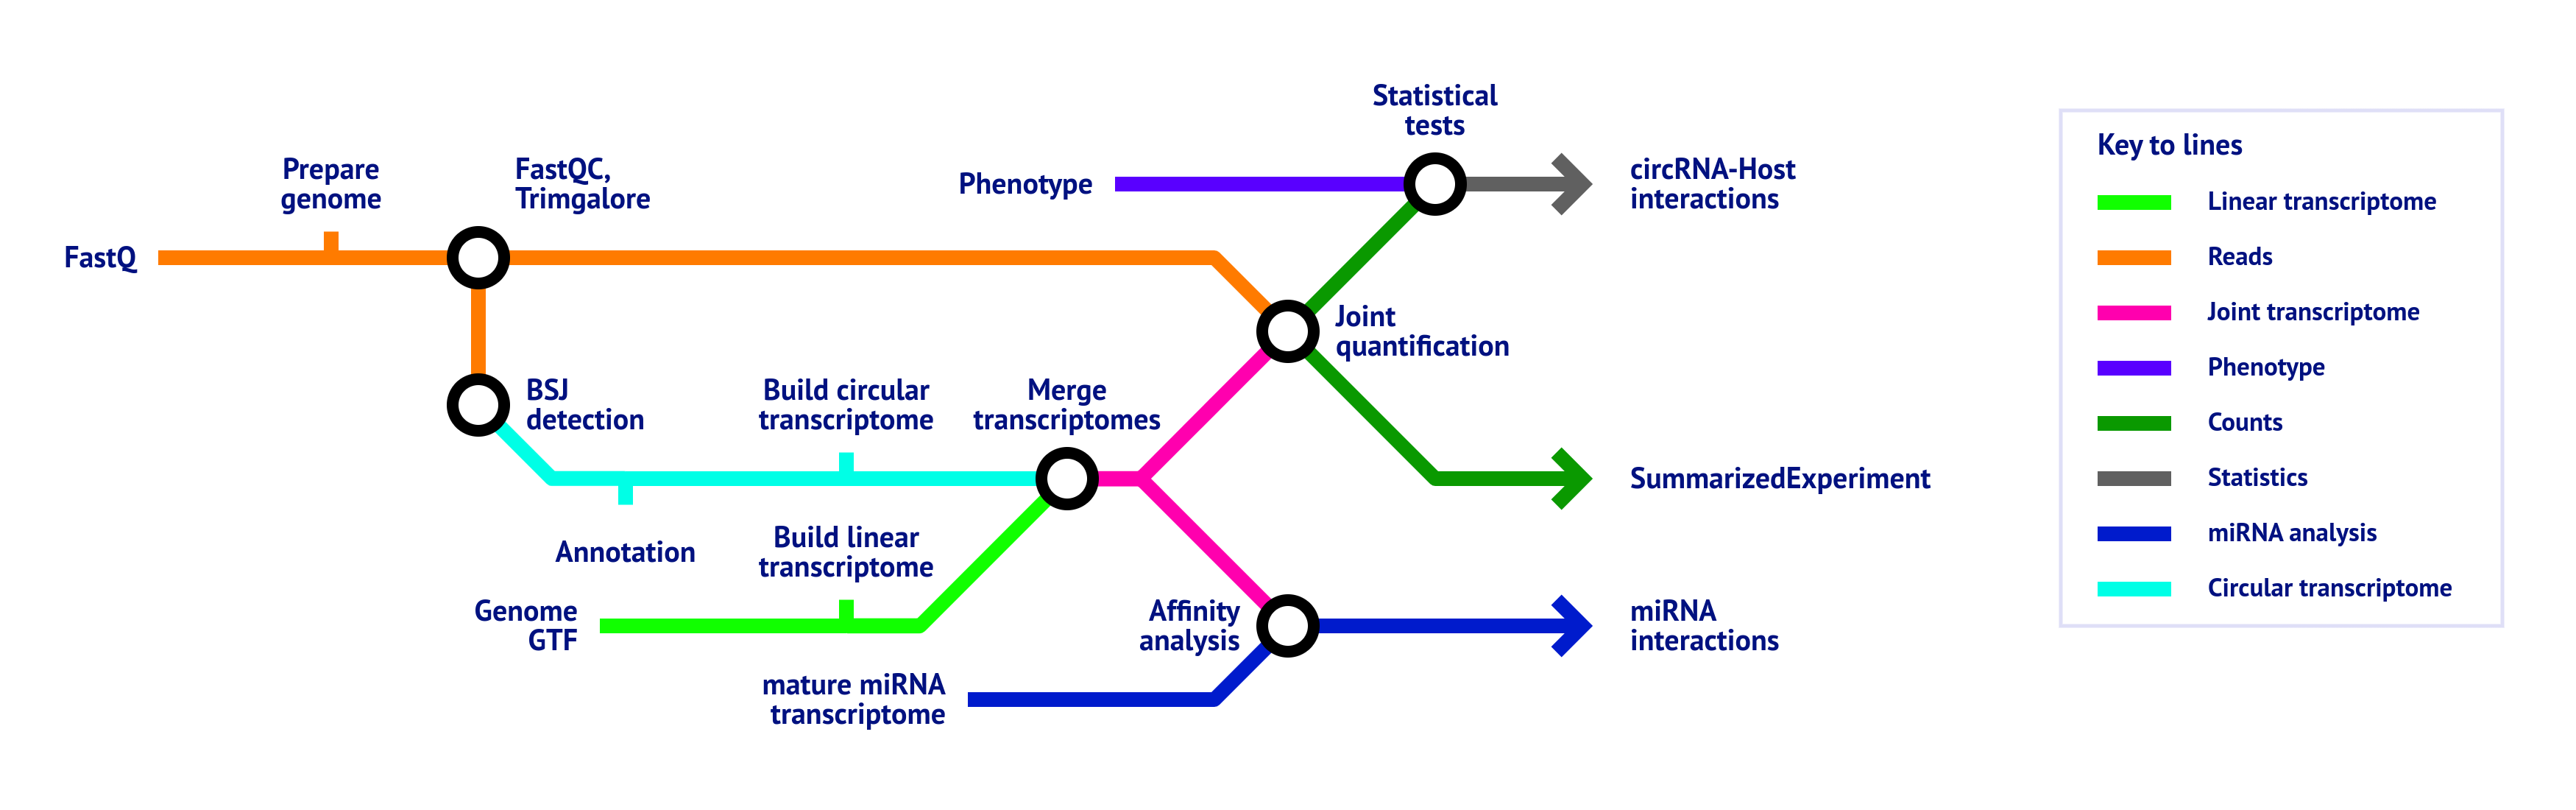
\includegraphics[width=\textwidth]{chapters/materials_and_methods/figures/nf-core_circrna.png}
    \caption{nf-core/circrna} % TODO: Add detailed caption
    \label{fig:circrna_pipeline}
\end{figure}

\subsection{circRNA detection}
What is the main task here?

\subsubsection{CIRIquant}
Describe CIRIquant

\subsubsection{CIRCexplorer2}
Describe CIRCexplorer2

\subsubsection{circRNA finder}
Describe circRNA finder

\subsubsection{DCC}
Describe DCC

\subsubsection{find\_circ}
Describe find circ

\subsubsection{MapSplice}
Describe MapSplice

\subsubsection{Segemehl}
Describe Segemehl

\subsection{circRNA annotation}
What is the main task here?

\subsubsection{GTF based annotation}
Describe GTF based annotation

\subsubsection{Database based annotation}
Describe database based annotation

\subsection{circRNA quantification}

Why is this important?

\subsubsection{psirc-quant}
Describe psirc-quant

\subsection{miRNA interaction analysis}
What can we learn from here?

\subsubsection{miRanda}
Describe miRanda

\subsubsection{TargetScan}
Describe TargetScan

\subsection{Downstream analyses}
\subsubsection{R-shiny}
\subsubsection{Dimensionality reduction}
\subsubsection{Pathway analysis}
\subsubsection{Differential expression analysis}
\subsubsection{Genome browser}
